\documentclass[a4paper]{article}
% \usepackage[a4paper]{geometry}
\usepackage{fullpage}
%\usepackage{cite}
\usepackage{times}
\usepackage{epsfig,endnotes}
%\usepackage{bibspacing}
%\setlength{\bibspacing}{\baselineskip}
%\usepackage{balance}
\usepackage{algorithm}
\usepackage{algorithmic}
\usepackage{amssymb,amsmath}
\usepackage{color}
\usepackage{comment}
\usepackage{multirow}
\usepackage{graphicx,subfigure}
\usepackage{url}
\usepackage{alltt}
\usepackage{listings}
\usepackage[normalem]{ulem}
\DeclareGraphicsExtensions{.pdf,.png,.jpg}
\lstset{basicstyle=\ttfamily\small, language=C, breaklines=true}


\begin{document}

\begin{centering}

\Large \Large \textbf{MCMR Design}\\
\small Weiwei Jia\\
\small www.jiaweiwei.com\\
\small Updated at Apr. 4, 2014\\

\end{centering}

\begin{flushleft}
\color{black}{\line(1, 0){450}}
\end{flushleft}

\section{Introduction}
MCMR is Mock Coffee Machine Running. Fig.~\ref{fig:mcmr-cm}[1]
shows the statecharts[2] of MCMR. This document aims to realize
a software to simulate what the statecharts says, which just
describes how coffee machine works well automatically.

\begin{figure}[htbp]
\begin{center}
  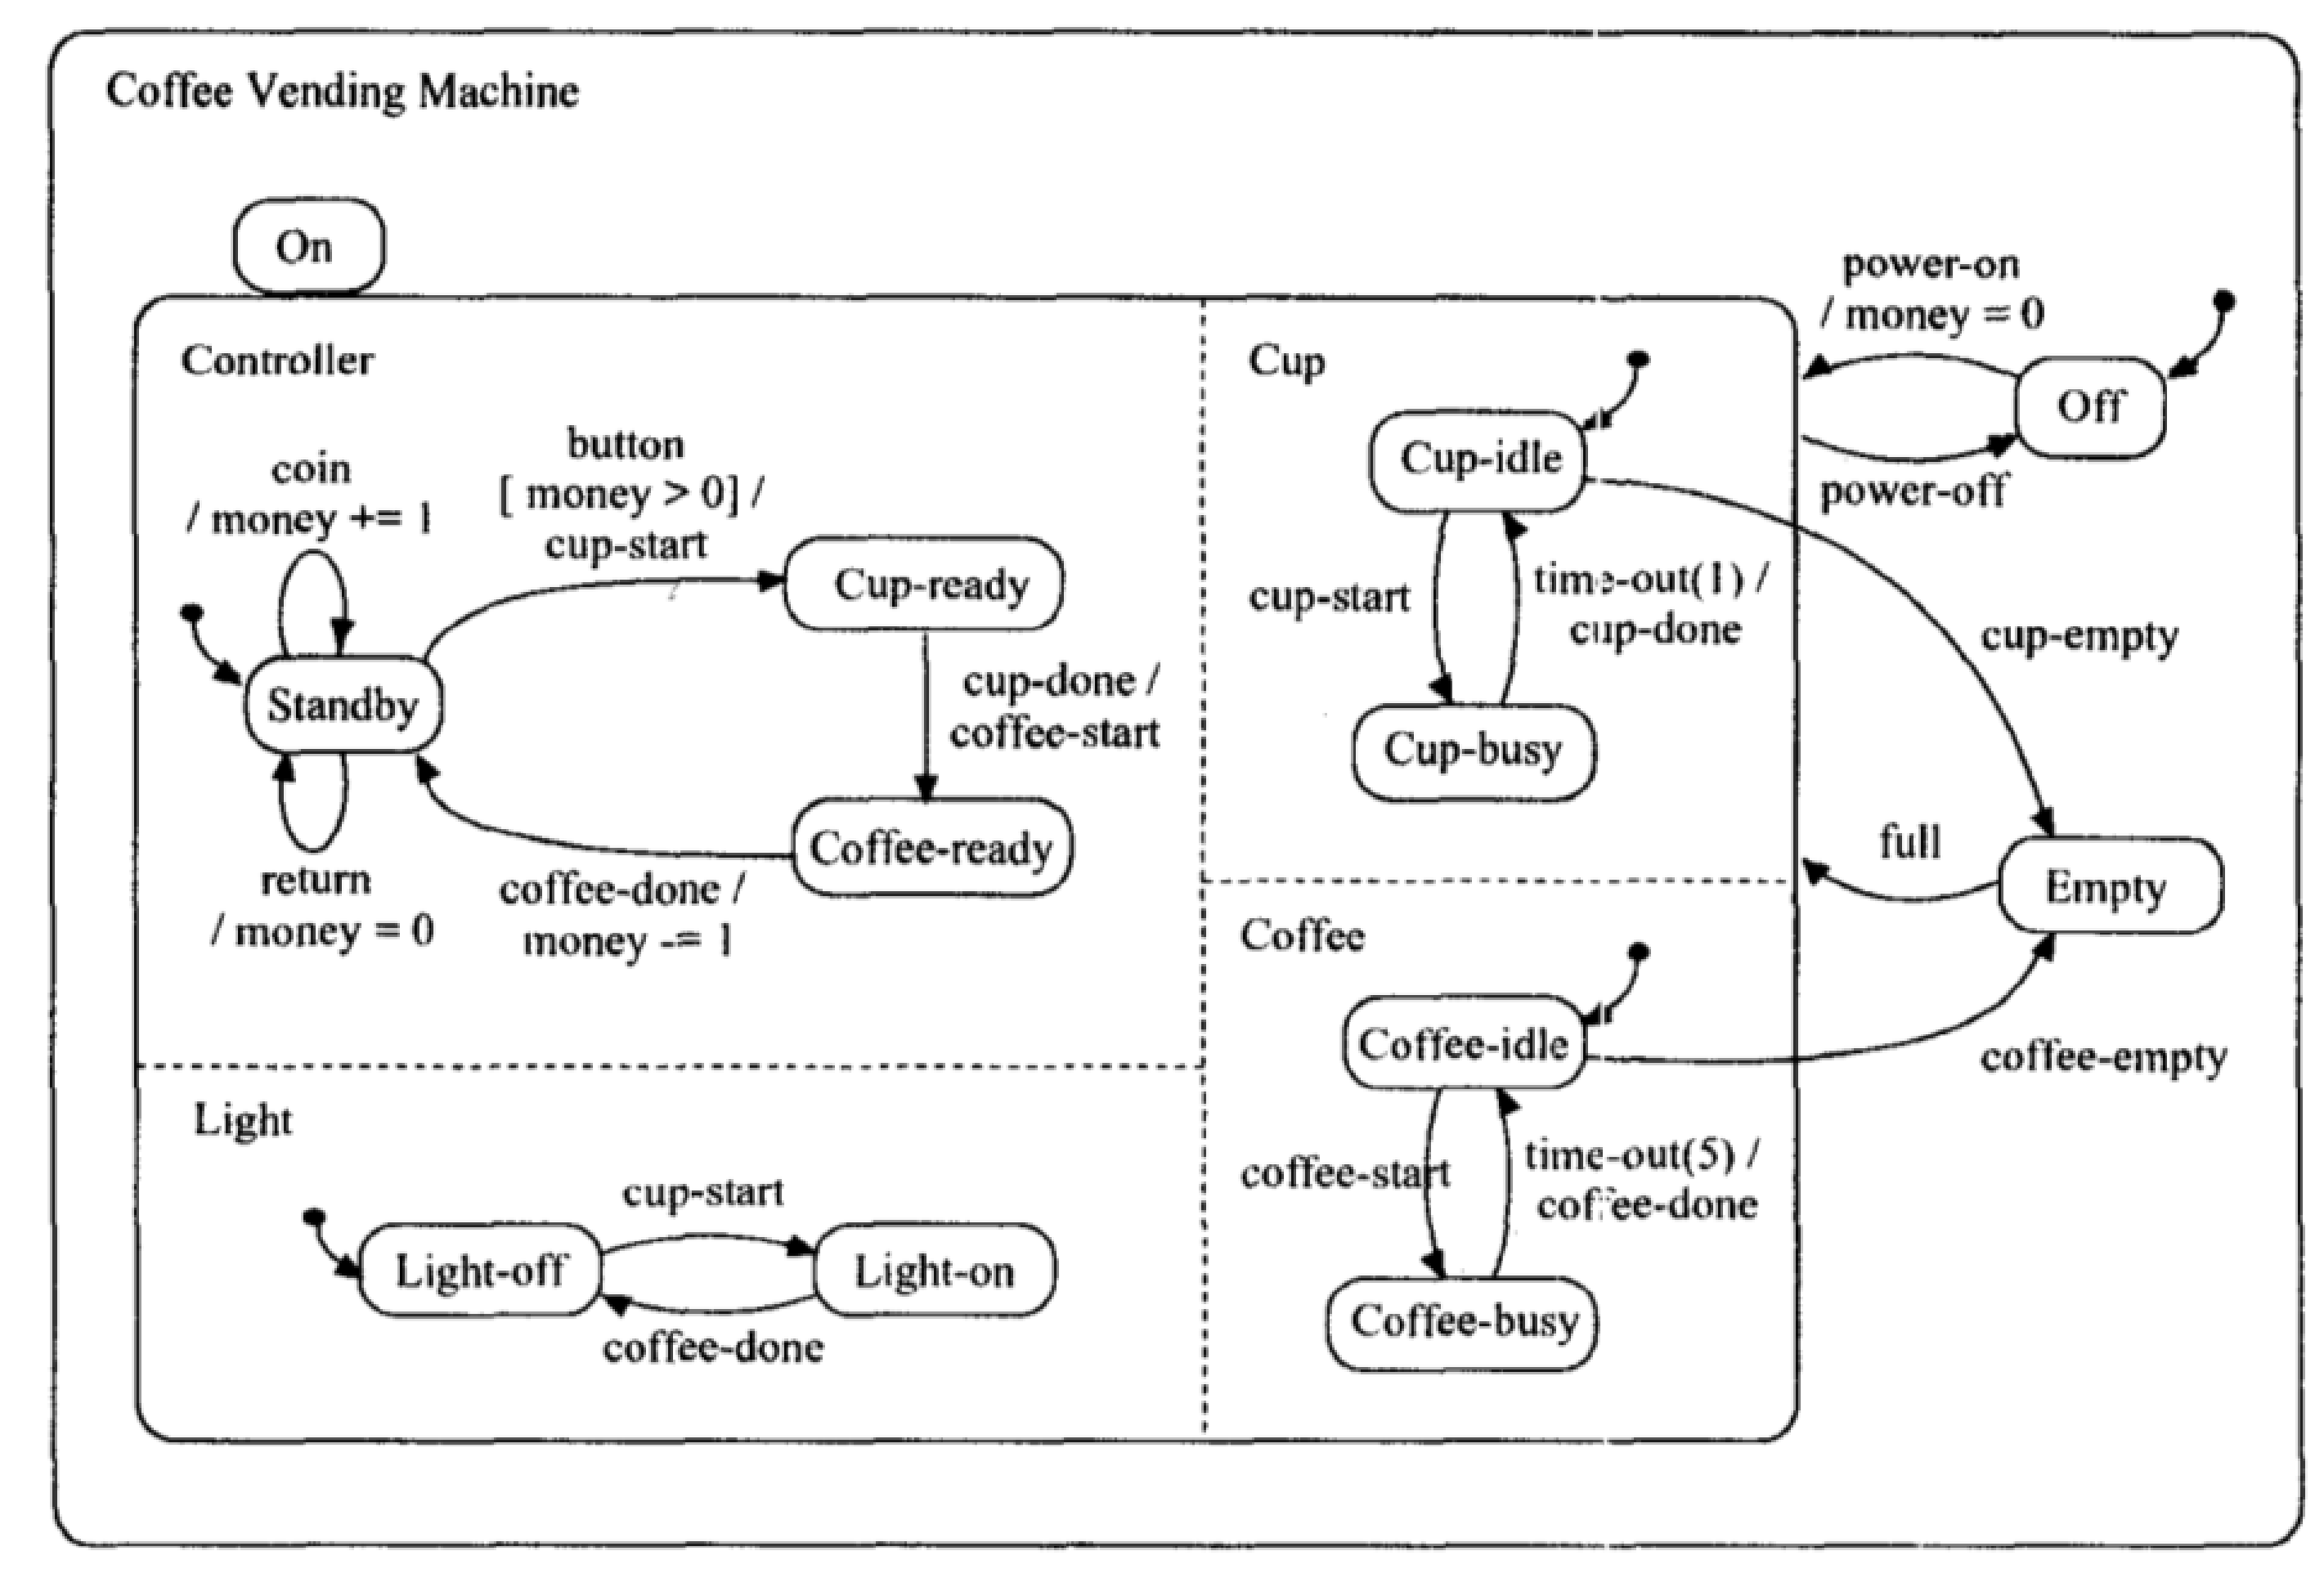
\includegraphics[width=5.8in]{figure/coffee_machine.eps}
  \caption{Mock Coffee Machine Running StateCharts}
  \label{fig:mcmr-cm}
\end{center}
\end{figure}

\section{General design}
As is seen from the statecharts diagram, there are three states
for the Coffee Vending Machine, which are `On`, `Off` and `Empty`.
`On` could transfer to `Off` when power-off is set. On the contrary,
`Off` turns to `On` after power is on and money is zero. Meanwhile,
`On` becomes `Empty` once cup/coffee is empty. `Empty` transfers to
`On` when cup/coffee is full. Actually, there are three conditions
for the transition between `On` and `Empty`.

\begin{itemize}
	\item Cup and Coffee are empty.
	\item Cup is empty and Coffee is not empty.
	\item Cup is not empty and Coffee is empty.
\end{itemize}

\subsection{Internal On state}
Once the Coffee Vending Machine is On, there would be four processes/threads
are started simultaneously, which are Controller process/thread, Light process/thread,
Cup process/thread and Coffee process/thread. Now, let's analyze each of them.


\begin{itemize}
	\item Controller process/thread\\
		\begin{enumerate}
			\item In Standby state in default. After one does coin action, money would plus one.
			\item After one does button action with money more than zero, it would transfer
				to Cup-ready state, which leads to cup-start (See Cup and Light processes/threads).
			\item After cup-done is set (See Cup process), Cup-ready would turn to Coffee-ready, which leads
				to coffee-start (See Coffee process).
			\item After coffee-done is set (See Coffee process), Coffee-ready would transfer to Standby
				state with money minus one.
			\item After one does return action, it transfers to Standby itself, which leads to money is zero.
		\end{enumerate}
	\item Cup process/thread\\
		\begin{enumerate}
			\item In Cup-idle state in default. After cup-start is set (in Controller process), it would transfer
				to Cup-busy.
			\item With one second duration, Cup-busy would turn to Cup-idle and cup-done is set in the same time.
			\item It would go to Empty state when there is no cup (cup-empty is set).
		\end{enumerate}
	\item Light process/thread\\
		\begin{enumerate}
			\item In Light-off state in default, it would become Light-on state with cup-start (Set in Controller process/thread).
			\item It would go back to Light-off state with coffee-done is set.
			\end{enumerate}
	\item Coffee process/thread\\
		\begin{enumerate}
			\item In Coffee-idle state in default. After coffee-start is set (in Controller process), it would transfer
				to Coffee-busy.
			\item With five seconds duration, Coffee-busy would turn to Coffee-idle and coffee-done is set in the same time.
			\item It would go to Empty state when there is no coffee (coffee-empty is set).
		\end{enumerate}
\end{itemize}


\section{Detail design}

\subsection{How MCMR works}
\begin{enumerate}
	\item Initialize corresponding stuffs, such as fields in the global memory control block and so on.
	\item The system is in Off state in default. Do power action, it goes to On state with money is initialized with zero.
	\item For rest parts, please see `Internal On State` section for details.
	\end{enumerate}

\subsection{How processes communicate with each other}
We use memory share technology in MCMR because it is faster.

\subsection{Related data structures}

The global data structure.
{\color{blue}{
\begin{verbatim}
-----------------------------------------------------------------------
struct mcmr {
	int money;
	int power_on;
	int power_off;
	int cup_empty;
	int cup_start;
	int cup_done;
	int coffee_empty;
	int coffee_start;
	int coffee_done;
	int time;
	struct coffee_vending_machine cvm;
	struct contorller controller;
	struct light light;
	struct cup cup;
	struct coffee coffee;
	struct action *do;
};
-----------------------------------------------------------------------
\end{verbatim}
}}

Actions Coffee Vending Machine does
{\color{blue}{
\begin{verbatim}
-----------------------------------------------------------------------
struct action {
	int (* coin) (struct mcmr *);
	int (* button) (struct mcmr *);
	int (* cup) (struct mcmr *);
	int (* coffee) (struct mcmr *);
	int (* time) (struct mcmr *);
	int (* power) (struct mcmr *);
	int (* return) (struct mcmr *);
};
-----------------------------------------------------------------------
\end{verbatim}
}}

The Coffee Vending Machine data structure
{\color{blue}{
\begin{verbatim}
-----------------------------------------------------------------------
struct coffee_vending_machine {
	int on;
	int off;
	int empty;
};
-----------------------------------------------------------------------
\end{verbatim}
}}

The Controller data structure
{\color{blue}{
\begin{verbatim}
-----------------------------------------------------------------------
struct controller{
	int standby;
	int cup_ready;
	int coffee_ready;
};
-----------------------------------------------------------------------
\end{verbatim}
}}

The Light data structure
{\color{blue}{
\begin{verbatim}
-----------------------------------------------------------------------
struct light {
	int light_off;
	int light_on;
}
-----------------------------------------------------------------------
\end{verbatim}
}}

The Cup data structure
{\color{blue}{
\begin{verbatim}
-----------------------------------------------------------------------
struct cup {
	int cup_idle;
	int cup_busy;
};
-----------------------------------------------------------------------
\end{verbatim}
}}

The Coffee data structure
{\color{blue}{
\begin{verbatim}
-----------------------------------------------------------------------
struct coffee {
	int coffee_idle;
	int coffee_busy;
};
-----------------------------------------------------------------------
\end{verbatim}
}}


\section{References}
[1] Hong, Hyoung Seok, et al. "Static semantics and priority schemes for statecharts." COMPSAC-NEW YORK- (1995): 114-114. \\\
[2] Harel, David. "Statecharts: A visual formalism for complex systems." Science of computer programming 8.3 (1987): 231-274.


\end{document}
